\documentclass[border=10pt]{standalone}
\usepackage[T1]{fontenc}
\usepackage[utf8]{inputenc}
\usepackage{amsmath}
\usepackage{graphicx}

\usepackage{tikz}
\usepackage{pgfplots}
\pgfplotsset{compat=1.18}

\usetikzlibrary{
    positioning,
    arrows.meta,
    shapes.geometric,
    shapes.misc,
    calc,
    backgrounds,
    fit,
    decorations.pathreplacing
}

% =============================================================================
% COLOR PALETTE
% =============================================================================
\definecolor{pretrainedblue}{RGB}{170, 205, 235}     % Pretrained (frozen)
\definecolor{learnedgreen}{RGB}{175, 215, 165}       % Learned (trainable)
\definecolor{functionorange}{RGB}{245, 190, 130}     % Data manipulation (no params)
\definecolor{inputgray}{RGB}{210, 210, 210}          % Inputs
\definecolor{backbonepurple}{RGB}{180, 160, 210}     % Pretrained backbone (fine-tuned)
\definecolor{outputyellow}{RGB}{240, 220, 120}       % Output
\definecolor{groupgray}{RGB}{230, 230, 230}
\definecolor{arrowblack}{RGB}{60, 60, 60}

% =============================================================================
% STYLES
% =============================================================================
\tikzset{
    base/.style={
        draw=arrowblack, align=center,
        minimum height=1.2cm, minimum width=3cm,
        line width=0.6pt, font=\small, rounded corners=2pt
    },
    inputbox/.style={base, fill=inputgray},
    pretrainedbox/.style={base, fill=pretrainedblue},
    learnedbox/.style={base, fill=learnedgreen},
    functionbox/.style={base, fill=functionorange},
    tokenpill/.style={
        draw=arrowblack!55, fill=learnedgreen!20,
        minimum width=0.46cm, minimum height=0.30cm,
        line width=0.45pt, rounded corners=2.8pt
    },
    backbonebox/.style={base, fill=backbonepurple, minimum width=4cm, minimum height=1.4cm, font=\normalsize\bfseries},
    outputbox/.style={base, fill=outputyellow},
    arr/.style={-Stealth, line width=0.8pt, draw=arrowblack},
    grouplabel/.style={font=\footnotesize, text=arrowblack!70},
    annot/.style={font=\scriptsize\itshape, text=arrowblack!60},
    paramcount/.style={font=\scriptsize, text=arrowblack!50}
}

\begin{document}
\begin{tikzpicture}

    % =========================================================================
    % LAYOUT
    %   Vision inputs are projected into image tokens and injected into the
    %   Gemma input stream. Joint state and task are formatted into text,
    %   tokenized, and injected into the same token stream from below.
    % =========================================================================

    % --- Vision branch ---
    \node[inputbox, minimum height=2.8cm] (images) at (5.45, 0.5)
        {Observations\\[2pt]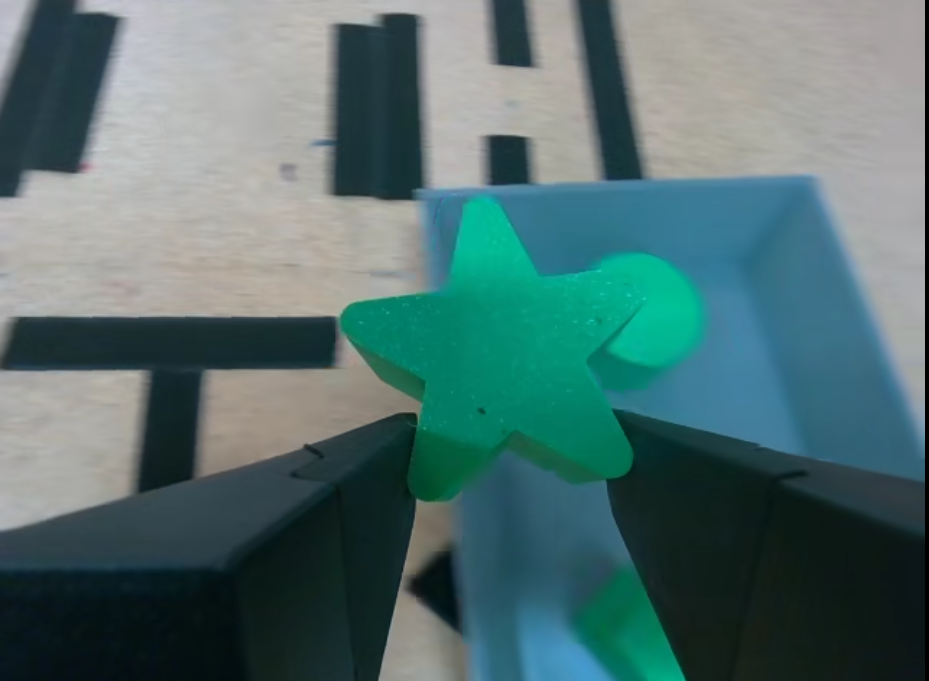
\includegraphics[width=2.1cm]{obs.png}\\[2pt]$\mathbf{o}_{t}$};
    \node[pretrainedbox] (siglip) at (9.95, 0.5) {Vision\\(SigLIP 400M)};
    \node[learnedbox]    (proj)   at (14.45, 0.5)   {Linear\\Projection};

    % --- Text branch ---
    \node[inputbox]      (joints) at (5.45, -3.1)  {Joint State\\$\mathbf{s}_{t}$};
    \node[inputbox]      (task)   at (5.45, -6.1)  {Task Description\\"pick up cup"};
    \node[functionbox]   (disc)   at (9.95, -3.1){Discretize\\(256 bins)};
    \node[functionbox]   (format) at (14.45, -3.1)  {Format\\Prompt};
    \node[pretrainedbox] (gemtok) at (18.95, -3.1) {Gemma Tokenizer\\+ Embedding};

    % --- Backbone and output ---
    \coordinate          (tokenstreamcenter) at (18, 3.75);
    \node[inner sep=0pt, minimum width=4.00cm, minimum height=0.30cm]
                         (tokenrow) at ($(tokenstreamcenter)+(0,-0.70)$) {};
    \foreach \dx in {-1.77, -1.18, -0.59, 0.00, 0.59, 1.18, 1.77} {
        \node[tokenpill] at ($(tokenrow.center)+(\dx,0)$) {};
    }
    \node[backbonebox]   (gemma)  at (18, 4.05)  {Gemma-3 270M};
    \node[functionbox]   (pool)   at (22.5, 4.05){Pool\\Last Token};
    \node[learnedbox]    (vhead)  at (26.5, 4.05){GELU MLP\\Value Head};
    \node[outputbox, inner sep=5pt, minimum height=0cm, minimum width=0cm] (bins) at (30.5, 4.05)
        {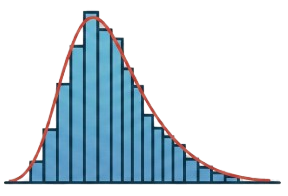
\includegraphics[width=2cm]{distribution.png}\\[-1pt]{\scriptsize Value Estimate}\\[-4pt]{\fontsize{6}{7}\selectfont Monte Carlo Distribution}};
    \coordinate (visiontokenin) at ($(tokenrow.center)+(-0.95, -0.40)$);
    \coordinate (texttokenin) at ($(tokenrow.center)+(0.95, -0.40)$);

    % =========================================================================
    % EDGES
    % =========================================================================

    % Vision: image tokens feed into the Gemma token stream
    \draw[arr] (images) -- (siglip);
    \draw[arr] (siglip) -- (proj);
    \draw[arr] (proj.east) -- (visiontokenin |- proj.east) -- (visiontokenin);

    % Text: state and task are turned into text tokens
    \draw[arr] (joints) -- (disc);
    \draw[arr] (disc) -- (format);
    \draw[arr] (task.east) -- (14.45, -6.1) -- (format.south);
    \draw[arr] (format) -- (gemtok);
    \draw[arr] (gemtok.north) -- (texttokenin |- gemtok.north) -- (texttokenin);

    % Backbone and prediction head
    \draw[arr] (gemma) -- (pool);
    \draw[arr] (pool) -- (vhead);
    \draw[arr] (vhead) -- (bins);

    % =========================================================================
    % BACKGROUND GROUPS
    % =========================================================================
    \begin{scope}[on background layer]
        \node[draw=arrowblack!30, rounded corners=5pt, fill=groupgray!50,
              fit=(siglip)(proj), inner sep=12pt,
              label={[grouplabel]above:Vision Pipeline}] {};
        \node[draw=arrowblack!30, rounded corners=5pt, fill=groupgray!50,
              fit=(disc)(format)(gemtok), inner sep=12pt,
              label={[grouplabel]above:"Task: pick up cup, State: 192 89 128 ...;"}] {};
        \node[draw=arrowblack!30, rounded corners=5pt, fill=groupgray!50,
              fit=(tokenrow)(gemma)(pool)(vhead)(bins), inner sep=12pt,
              label={[grouplabel]above:Value Prediction}] {};
    \end{scope}

    % =========================================================================
    % LEGEND (bottom right)
    % =========================================================================
    \node[anchor=north west, font=\footnotesize\bfseries] (ltitle) at (21.8, -1.8) {Legend};
    \draw[arrowblack!40, line width=0.4pt] (ltitle.south west) -- ++(8.5, 0);

    \node[fill=pretrainedblue, draw=arrowblack, minimum width=0.5cm, minimum height=0.5cm,
          rounded corners=2pt, line width=0.4pt,
          anchor=north west] (l1) at ($(ltitle.south west) + (0, -0.3)$) {};
    \node[font=\scriptsize, right=0.2cm of l1] {Pretrained (frozen)};

    \node[fill=learnedgreen, draw=arrowblack, minimum width=0.5cm, minimum height=0.5cm,
          rounded corners=2pt, line width=0.4pt, below=0.25cm of l1] (l2) {};
    \node[font=\scriptsize, right=0.2cm of l2] {Learned (trainable)};

    \node[fill=backbonepurple, draw=arrowblack, minimum width=0.5cm, minimum height=0.5cm,
          rounded corners=2pt, line width=0.4pt, below=0.25cm of l2] (l3) {};
    \node[font=\scriptsize, right=0.2cm of l3] {Pretrained backbone (fine-tuned)};

    \node[fill=functionorange, draw=arrowblack, minimum width=0.5cm, minimum height=0.5cm,
          rounded corners=2pt, line width=0.4pt, below=0.25cm of l3] (l4) {};
    \node[font=\scriptsize, right=0.2cm of l4] {Data manipulation (no parameters)};

    \node[fill=inputgray, draw=arrowblack, minimum width=0.5cm, minimum height=0.5cm,
          rounded corners=2pt, line width=0.4pt, below=0.25cm of l4] (l5) {};
    \node[font=\scriptsize, right=0.2cm of l5] {Input};

    \node[fill=outputyellow, draw=arrowblack, minimum width=0.5cm, minimum height=0.5cm,
          rounded corners=2pt, line width=0.4pt, below=0.25cm of l5] (l6) {};
    \node[font=\scriptsize, right=0.2cm of l6] {Output};

\end{tikzpicture}
\end{document}
